\section{Factor Loadings under Input Ablations}
\label{app:ablation-factor}

The factor-prior interpretation in Section~\ref{sec:factor} asks not only whether LLM rankings have alpha, but \emph{which information channel} generates the implicit ranking profile.

Table~\ref{tab:ablation-ff6} reports FF6 loadings and alphas under fundamentals-only, market-only, and full-input settings for o3, Gemini 2.5 Pro, and Claude Opus 4.
Table~\ref{tab:ablation-char} reports the corresponding within-universe style fingerprint for the same representative models.
Figure~\ref{fig:ablation-ff6} visualizes how factor exposures shift when fundamentals or market summaries are removed.

Two patterns emerge.
First, \textbf{market-only inputs preserve most of the full-input factor profile}: positive momentum and negative value/profitability/investment loadings remain for the strongest models, consistent with the hypothesis-test result that full-input and market-only performance are not significantly different.
Second, \textbf{fundamentals-only inputs weaken both alpha and style coherence}: some FF6 market and momentum exposure remains, but alpha collapses and characteristic fingerprints become noisier, indicating that sparse accounting panels alone do not sustain a stable economically useful factor-like prior in this universe.

\begin{table}[H]
\centering
\caption{FF6 factor loadings of representative Q1$-$Q5 portfolios under input ablations. $\alpha$ is annualized percent; stars use Newey--West HAC SE.}
\label{tab:ablation-ff6}
\scriptsize
\setlength{\tabcolsep}{2.5pt}
\resizebox{\textwidth}{!}{
\begin{tabular}{llrllllllr}
\toprule
\textbf{Model} & \textbf{Input} & $\alpha$ & $\beta_{\text{MKT}}$ & $\beta_{\text{SMB}}$ & $\beta_{\text{HML}}$ & $\beta_{\text{RMW}}$ & $\beta_{\text{CMA}}$ & $\beta_{\text{MOM}}$ & $R^2_{\text{adj}}$ \\
\midrule
o3 & Fund. + Market & 127.7 & +0.86$^{***}$ & -0.06 & -0.70$^{***}$ & -0.60$^{**}$ & +0.28 & +0.34$^{**}$ & 0.45 \\
o3 & Market only & 156.5 & +0.76$^{***}$ & +0.20 & -0.81$^{***}$ & -0.36 & +0.38 & +0.68$^{***}$ & 0.48 \\
o3 & Fund. only & 39.7 & +0.68$^{***}$ & +0.05 & -0.82$^{***}$ & -0.36 & +0.24 & +0.67$^{***}$ & 0.44 \\
\midrule
Gem. 2.5 Pro & Fund. + Market & 87.6 & +0.83$^{***}$ & -0.06 & -0.64$^{***}$ & -0.75$^{***}$ & +0.40 & +0.51$^{***}$ & 0.38 \\
Gem. 2.5 Pro & Market only & 116.8 & +1.02$^{***}$ & -0.43 & -0.86$^{***}$ & -0.43 & +0.85$^{***}$ & +0.32 & 0.42 \\
Gem. 2.5 Pro & Fund. only & 24.9 & +0.50$^{***}$ & -0.00 & -0.97$^{***}$ & -0.30 & +0.48$^{**}$ & +0.66$^{***}$ & 0.44 \\
\midrule
Cl. Opus 4 & Fund. + Market & 129.6 & +0.68$^{***}$ & -0.06 & -0.18 & -0.42 & -0.06 & +0.59$^{***}$ & 0.26 \\
Cl. Opus 4 & Market only & 143.6 & +0.58$^{***}$ & +0.16 & -0.78$^{***}$ & -0.44$^{*}$ & +0.97$^{***}$ & +0.79$^{***}$ & 0.44 \\
Cl. Opus 4 & Fund. only & 12.2 & +0.55$^{***}$ & -0.07 & -0.96$^{***}$ & -0.32$^{*}$ & +0.26 & +0.76$^{***}$ & 0.56 \\
\bottomrule
\end{tabular}
}
\end{table}


\begin{table}[H]
\centering
\caption{Within-universe style fingerprint under input ablations. Values are average Q1$-$Q5 normalized characteristic ranks; stars test the monthly mean spread with Newey--West HAC SE: $^{*}p<0.10$, $^{**}p<0.05$, $^{***}p<0.01$.}
\label{tab:ablation-char}
\scriptsize
\setlength{\tabcolsep}{3pt}
\resizebox{\textwidth}{!}{
\begin{tabular}{ll llllll}
\toprule
\textbf{Model} & \textbf{Input} & Mom & Rev & LowVol & E/P & ROE & LowInv \\
\midrule
o3 & Fund. + Market & +0.04 & \multicolumn{1}{l}{-0.21$^{*}$} & \multicolumn{1}{l}{-0.57$^{***}$} & \multicolumn{1}{l}{-0.21$^{***}$} & \multicolumn{1}{l}{-0.05$^{***}$} & \multicolumn{1}{l}{-0.10$^{***}$} \\
o3 & Market only & \multicolumn{1}{l}{+0.17$^{**}$} & \multicolumn{1}{l}{-0.23$^{**}$} & \multicolumn{1}{l}{-0.48$^{***}$} & \multicolumn{1}{l}{-0.33$^{***}$} & \multicolumn{1}{l}{-0.15$^{***}$} & \multicolumn{1}{l}{-0.20$^{***}$} \\
o3 & Fund. only & +0.15 & -0.13 & \multicolumn{1}{l}{-0.47$^{***}$} & \multicolumn{1}{l}{-0.37$^{***}$} & \multicolumn{1}{l}{-0.06$^{**}$} & \multicolumn{1}{l}{-0.21$^{***}$} \\
\midrule
Gem. 2.5 Pro & Fund. + Market & \multicolumn{1}{l}{+0.24$^{***}$} & \multicolumn{1}{l}{-0.22$^{**}$} & \multicolumn{1}{l}{-0.52$^{***}$} & \multicolumn{1}{l}{-0.41$^{***}$} & \multicolumn{1}{l}{-0.29$^{***}$} & \multicolumn{1}{l}{-0.12$^{**}$} \\
Gem. 2.5 Pro & Market only & \multicolumn{1}{l}{+0.23$^{**}$} & -0.10 & \multicolumn{1}{l}{-0.38$^{***}$} & \multicolumn{1}{l}{-0.30$^{**}$} & \multicolumn{1}{l}{-0.05$^{**}$} & \multicolumn{1}{l}{-0.15$^{***}$} \\
Gem. 2.5 Pro & Fund. only & +0.21 & -0.04 & \multicolumn{1}{l}{-0.37$^{***}$} & \multicolumn{1}{l}{-0.43$^{***}$} & +0.01 & \multicolumn{1}{l}{-0.23$^{***}$} \\
\midrule
Cl. Opus 4 & Fund. + Market & \multicolumn{1}{l}{+0.32$^{***}$} & \multicolumn{1}{l}{-0.16$^{***}$} & \multicolumn{1}{l}{-0.35$^{***}$} & \multicolumn{1}{l}{-0.31$^{***}$} & \multicolumn{1}{l}{-0.13$^{*}$} & \multicolumn{1}{l}{-0.23$^{***}$} \\
Cl. Opus 4 & Market only & \multicolumn{1}{l}{+0.23$^{**}$} & \multicolumn{1}{l}{-0.13$^{*}$} & \multicolumn{1}{l}{-0.43$^{***}$} & \multicolumn{1}{l}{-0.36$^{***}$} & \multicolumn{1}{l}{-0.04$^{**}$} & \multicolumn{1}{l}{-0.15$^{***}$} \\
Cl. Opus 4 & Fund. only & \multicolumn{1}{l}{+0.40$^{***}$} & \multicolumn{1}{l}{-0.11$^{**}$} & \multicolumn{1}{l}{-0.38$^{***}$} & \multicolumn{1}{l}{-0.46$^{***}$} & \multicolumn{1}{l}{+0.10$^{**}$} & \multicolumn{1}{l}{-0.32$^{***}$} \\
\bottomrule
\end{tabular}
}
\end{table}


\begin{figure}[H]
  \centering
  \IfFileExists{figures/fig10_ablation_ff6_loadings.pdf}{%
    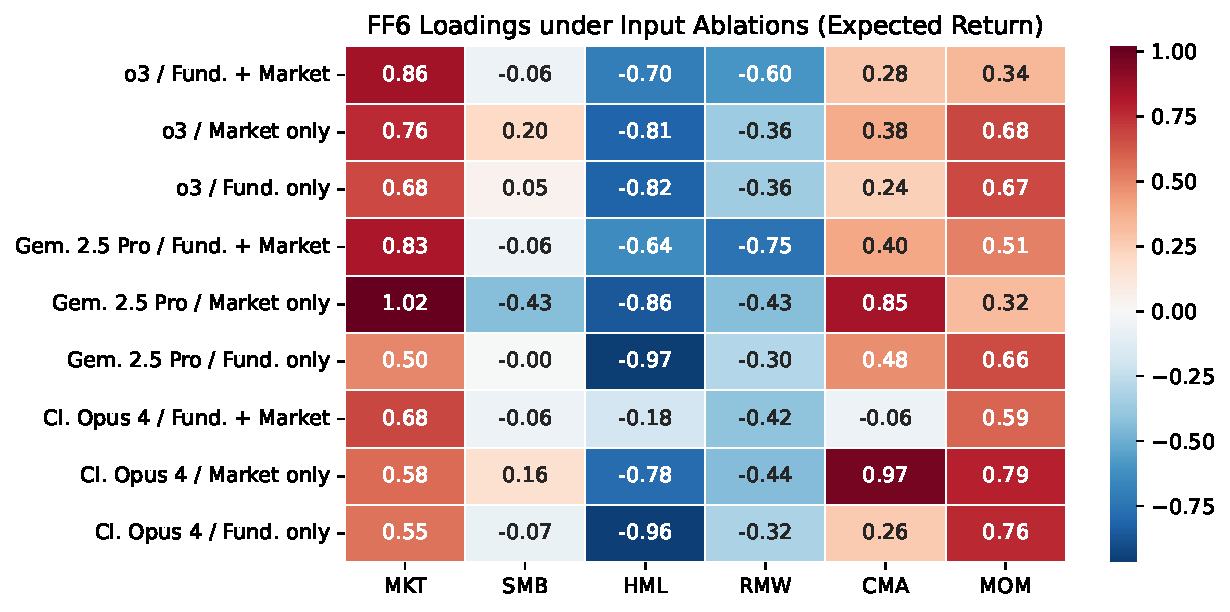
\includegraphics[width=0.86\textwidth]{figures/fig10_ablation_ff6_loadings.pdf}%
  }{%
    \fbox{\parbox{0.9\textwidth}{\centering\vspace{2em}Run \texttt{python3 scripts/evaluate\_ablation\_factor\_loadings.py} to generate \texttt{figures/fig10\_ablation\_ff6\_loadings.pdf}.\vspace{2em}}}%
  }
  \caption{FF6 factor loadings of representative Q1$-$Q5 portfolios under input ablations. Red indicates positive loading and blue indicates negative loading.}
  \Description{Heatmap of Fama-French six-factor loadings for three representative models under fundamentals-only, market-only, and full-input settings, with color indicating loading sign and magnitude.}
  \label{fig:ablation-ff6}
\end{figure}

% ──────────────────────────────────────────────────────────────
\clearpage
